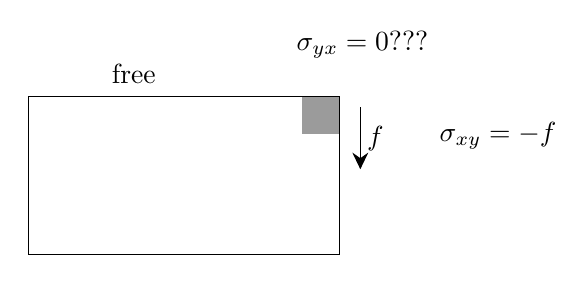
\begin{tikzpicture}[x=0.75pt,y=0.75pt,yscale=-1,xscale=1]
    %uncomment if require: \path (0,300); %set diagram left start at 0, and has height of 300
    
    %Shape: Rectangle [id:dp5412398632290694] 
    \draw   (98,59.94) -- (247.83,59.94) -- (247.83,136) -- (98,136) -- cycle ;
    %Straight Lines [id:da2034092160028942] 
    \draw    (258,65) -- (258,91.94) ;
    \draw [shift={(258,94.94)}, rotate = 270] [fill={rgb, 255:red, 0; green, 0; blue, 0 }  ][line width=0.08]  [draw opacity=0] (8.04,-3.86) -- (0,0) -- (8.04,3.86) -- (5.34,0) -- cycle    ;
    %Shape: Square [id:dp9141897458105774] 
    \draw  [draw opacity=0][fill={rgb, 255:red, 155; green, 155; blue, 155 }  ,fill opacity=1 ] (229.83,59.94) -- (247.83,59.94) -- (247.83,77.94) -- (229.83,77.94) -- cycle ;
    
    % Text Node
    \draw (260,79.97) node [anchor=west] [inner sep=0.75pt]    {$f$};
    % Text Node
    \draw (148.88,55) node [anchor=south] [inner sep=0.75pt]   [align=left] {free};
    % Text Node
    \draw (295,71) node [anchor=north west][inner sep=0.75pt]    {$\sigma _{xy} =-f$};
    % Text Node
    \draw (226,27) node [anchor=north west][inner sep=0.75pt]   [align=left] {$\displaystyle \sigma _{yx} =0$???};
    
    
    \end{tikzpicture}
    